\documentclass{article}
\usepackage[utf8]{inputenc}
\usepackage[margin=1in]{geometry}
\usepackage{graphicx}

\title{ORIE 4741 Midterm Project Proposal}
\author{Nehal Rawat (nr338) and Nihar Sidhu (ns625) }
\date{October 26, 2017}

\begin{document}

\maketitle

\section{Introduction}
For our project, we are looking at The Statewide Planning and Research Cooperative System (SPARCS) dataset. This dataset has information about patients receiving treatment at various hospitals across New York state in 2012. Features in the dataset include New York state counties, demographics such as the age and race of patients, length of stay of a patient at the hospital, total costs, and total charges. Our goal is to gain some insight into what factors, and how, they affect hospital costs across New York State, and create a model that can predict an individual’s hospital costs based on these input factors. 

\section{Describing the Dataset}
Our dataset is quite large - it has around 2.5 million entries with 37 features. Some entries in the dataset are missing, specifically for abortion cases. Therefore, when developing our models, we have decided to ignore these entries. Out of the 37 features, we have decided to focus on the following 11 features: 

\begin{enumerate}
\setlength{\itemsep}{1pt}
  \item Hospital County: To condense our data, we are looking at counties in New York State that vary in their locations (rural vs. urban) and socioeconomically. Specifically, we have decided to focus our analysis on Westchester (in Hudson Valley area and has 2nd highest per capita income in NY) and the Bronx (in New York City and has the 62nd and lowest pre-capita income in NY). As we continue to look at our data, we may also look at counties such as Oneida or Niagara that are in the middle of the per capita income range in NY.
  \item Age Group (at the time of discharge): The dataset already groups ages into 0 to 17, 8 to 29, 30 to 49, 50 to 69, and 70 or older.
  \item Gender: Patient gender is wither (M) Male, (F) Female, or (U) Unknown.
  \item Race: Patient race either Black/African American, Multi, Other Race, Unknown, White. Other Race includes Native Americans and Asian/Pacific Islander.
  \item Ethnicity: Patient ethnicity either Spanish/Hispanic Origin, Not of Spanish/Hispanic Origin, Multi, or Unknown.
  \item  Length of stay in days: The total number of patient days at an acute level and/or other than acute care level (excluding leave of absence days)
  \item Type of Admission (Elective or Urgency): A description of the manner in which the patient was admitted to the health care facility: Elective, Emergency, Newborn, Not Available, Trauma, Urgent.
  \item CCS Diagnosis Description: This column is especially of interest because now we don’t have to worry about the nominal diagnoses data – we can pull a lot the data from this code based column. We plan to use this column to investigate how costs compare across various illnesses. 
  \item APR Severity of Illness Code: “All Patients Refined” Code gives severity levels (1 – minor, 2 – moderate, 3 – major, 4 – extreme). An interesting feature would be to see if severity alone has any correlation between the hospital costs.
  \item Total Costs
\end{enumerate}

After analyzing our dataset, we decided to focus on the comparisons between counties, and how costs are affected by this factor, as mentioned above. We started by looking at the Westchester subset, which has 127212 entries and 9 features (as mentioned above, not including Hospital County), and calculating total cost statistics:
\begin{itemize}
\setlength{\itemsep}{1pt}
  \item Average Total Hospital Cost = \$13,419.41 
  \item Minimum Total Hospital Cost = \$10.62 
  \item Maximum Total Hospital Cost = \$1,623,714.74 
\end{itemize}
We created graphs to depict the nature of our data. Three of the graphs we produced showing age groups, races, and hospital cost versus illness severity are shown below:

\begin{figure}[h]
  \centering
  \begin{minipage}[b]{0.4\textwidth}
    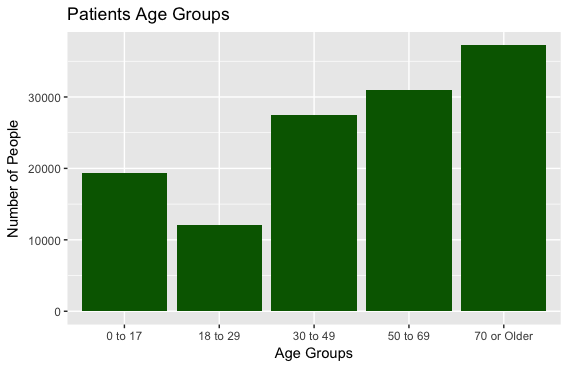
\includegraphics[width=\textwidth]{patientsAge.png}
    \caption{Comparing Age Demographic}
  \end{minipage}
  \hfill
  \begin{minipage}[b]{0.4\textwidth}
    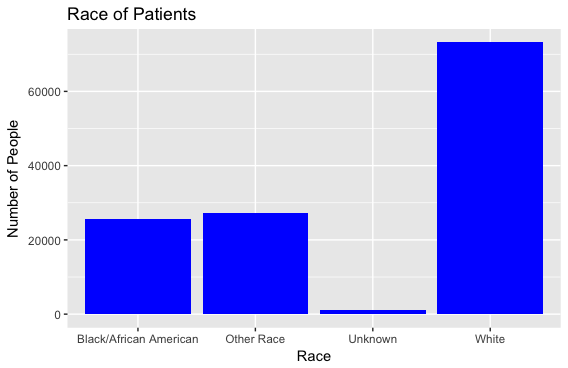
\includegraphics[width=\textwidth]{race.png}
    \caption{Comparing Race Demographic}
  \end{minipage}
\end{figure}


\begin{figure}[h]
\centering
  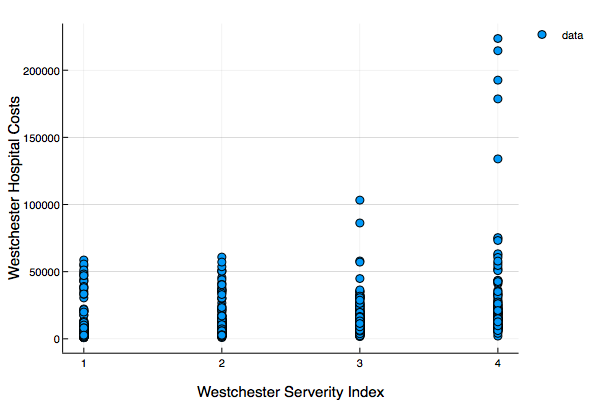
\includegraphics[width=8cm]{newplot.png}
  \label{fig:boat1}
  \caption{Comparing Hospital Costs and Illness Severity}
\end{figure}

\section{Developing Predictive Models}

\subsection{Data Cleaning and Feature Transformation}
Some of our entries in the dataset are incomplete. These entries are abortion cases as specified by the dataset provider. As the dataset is overall comprehensive with minimal missing values, we decided to remove these entries.We utilized one-hot encoding to transform categorical features into vectors of 0's and 1's, which will help improve the accuracy of our model, as most of our features are categorical.\newline \newline
We then attempted to understand the correlation between our features. We removed the CCS Diagnosis Description from this comparison, as the patient condition description cannot be transformed into a numerical value. We developed a correlation plot shows the correlation between our features. We saw that the features we selected were actually not highly correlated, therefore within this set of selected features, we do not need to reduce dimension. The correlation plot is shown below:

\begin{figure}[h]
\centering
  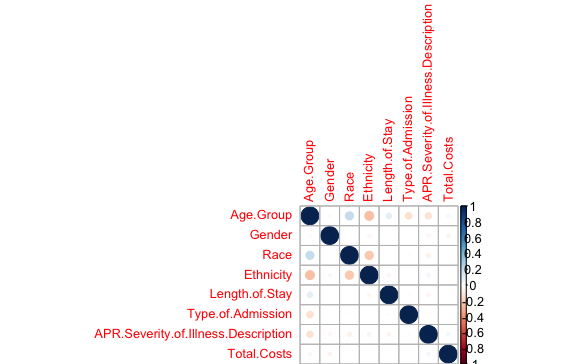
\includegraphics[width=8cm]{Rplot.png}
  \label{fig:boat1}
\end{figure}


\subsection{Preliminary Models}

We started by attempting to fit a linear model to predict hospital costs based on the features described above. We divided our data into a training set (consisting 80\% of the data) and a test set (consisting 20\% of the data). We developed the linear regression model using the training set, and applied the model on the test set to determine the accuracy of our cost predictions. The results of our analysis can be seen below:

\begin{figure}[h]
\centering
  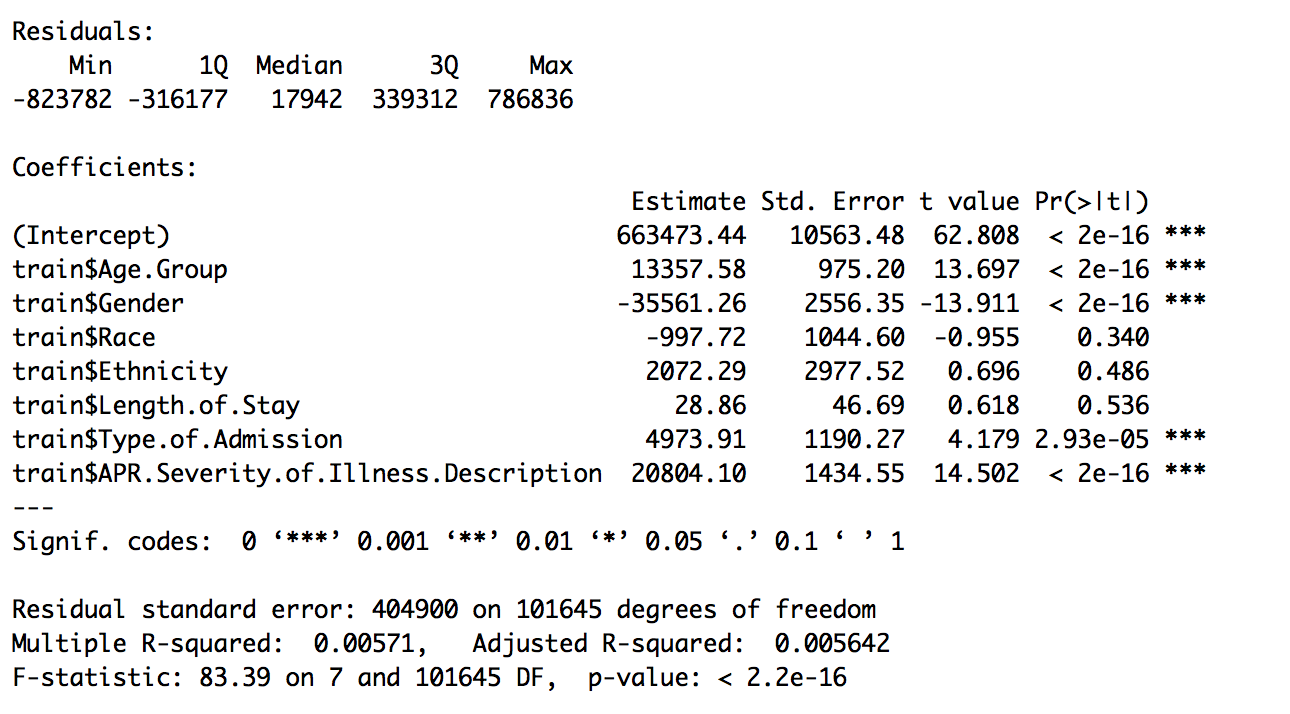
\includegraphics[width=12cm]{results.png}
  \label{fig:boat1}
\end{figure}

We can see that our model is not yet accurate, and we need to work on improving the model so it does not underfit the data.


\section{Moving Forward}
Moving forward, there are a couple of things we need to do. We need to create a better polynomial model that can help us determine hospital costs in the Westchester and Bronx counties. Currently, we are looking at the features such as length of stay, age, and severity illness to predict hospital costs. However, we can perhaps get a more accurate model by going deeper into the types of illnesses. For example, our model may be more accurate if we look into the hospital costs for pneumonia in Westchester or Bronx. If we decide to look at illnesses specifically, we will have to clean our data and make sure we have enough data within each categorical illness to train and test our models on.  




\end{document}
